%----------- Necessary Style Preamble -----------%

\documentclass[mathserif, 10pt]{beamer} %

\usepackage[framesassubsections]{beamerprosper}
\usepackage{beamerthemesplit} % Activate for custom appearance
\usepackage[english]{babel}
\usepackage[latin1]{inputenc}
\usepackage{amsmath, hyperref, subfigure, multirow, rotating}
\usepackage{epstopdf}
\usepackage{verbatim}
\usepackage{listings}
\usepackage{color}
\usepackage{esint}
\usepackage{mathrsfs}
\usepackage{multicol}

%\usepackage{enumitem}

\usetheme{Frankfurt}
\usecolortheme{default}
\usecolortheme[rgb={0.1,0.4,0.0}]{structure} % CSU color style
%\usecolortheme[rgb={0.541,0.149,0.196}]{structure} % BME color style

\setbeamersize{text margin left=0.5cm}
\setbeamersize{text margin right=0.5cm}

\setbeamercovered{transparent}

\usepackage{remreset}
\makeatletter
\@removefromreset{subsection}{section}
\makeatother
\setcounter{subsection}{1}

\makeatletter
\newcommand\xleftrightarrow[2][]{\ext@arrow 0099{\longleftrightarrowfill@}{#1}{#2}}
\def\longleftrightarrowfill@{\arrowfill@\leftarrow\relbar\rightarrow}
\makeatother


\newcommand\Wider[2][3em]{%
\makebox[\linewidth][c]{%
  \begin{minipage}{\dimexpr\textwidth+#1\relax}
  \raggedright#2
  \end{minipage}%
  }%
}

%----------- Math Definitions -----------%

\definecolor{Blue}{rgb}{0,0,1}
\def\ci{\perp\!\!\!\perp}
\def\a{\mathbf{a}}
\def\d{\mathbf{d}}
\def\e{\mathbf{e}}
\def\f{\mathbf{f}}
\def\g{\mathbf{g}}
\def\b{\mathbf{b}}
\def\q{\mathbf{q}}
\def\v{\mathbf{v}}
\def\x{\mathbf{x}}
\def\y{\mathbf{y}}
\def\u{\mathbf{u}}
%\def\z{\mathbf{\mathfrak{z}}}
\def\z{\mathbf{z}}
\def\D{\mathbf{D}}
\def\S{\mathbf{S}}
\def\X{\mathbf{X}}
\def\Z{\mathbf{Z}}
\def\1{\raisebox{.5pt}{\textcircled{\raisebox{-.9pt} {1}}}}
\def\2{\raisebox{.5pt}{\textcircled{\raisebox{-.9pt} {2}}}}
\def\3{\raisebox{.5pt}{\textcircled{\raisebox{-.9pt} {3}}}}
\def\4{\raisebox{.5pt}{\textcircled{\raisebox{-.9pt} {4}}}}
\def\5{\raisebox{.5pt}{\textcircled{\raisebox{-.9pt} {5}}}}
\def\6{\raisebox{.5pt}{\textcircled{\raisebox{-.9pt} {6}}}}
\def\balph{\boldsymbol\alpha}
\def\bmu{\boldsymbol\mu}
\def\btheta{\boldsymbol\theta}
\def\bomega{\boldsymbol\omega}
\def\bDelta{\boldsymbol\Delta}

%----------- Title Page Parameters -----------%
\title[Digital Control \& Digital Filters]{Digital Controls \& Digital Filters \\ Lectures 21 \& 22}
\author[M.R. Azimi]{M.R. Azimi, Professor}
\institute[CSU-ECE]{Department of Electrical and Computer Engineering \\ Colorado State University}
\date{Spring 2015}

\logo{
\includegraphics[height=0.5cm]{csu-logo.png}}

\newcommand{\unt}[1]{ \mathrm{\ #1}}

\begin{document}

%----------- slide --------------------------------------------------%

\frame{\titlepage}

\section{Analog Filter Design}
%----------- slide --------------------------------------------------%
\frame
{
%\vspace{-.2in}
\small
%\renewcommand{\theenumi}{\alph{enumi}}
\frametitle{Review of Analog Filters-Cont.}
\textcolor{red}{Types of Analog Filters:}\\
\begin{enumerate}
	\item Butterworth
	\item Chebyshev
	\item Elliptic (Cauer)
	\item Bessel
\end{enumerate}

Narrower Transition: (1) Elliptic, (2) Chebyshev, (3) Butterworth, (4) Bessel \\ \vspace{.05in}
More linear phase over PB: (1) Bessel, (2) Butterworth,  (3) Chebyshev, (4) Elliptic \\ \vspace{.1in}

\small
The first three filters have a common form of magnitude-squared function:\\ \vspace{.05in}
$A_N(\tilde\omega^2) = \frac{1}{1+F(\tilde\omega^2)}$\\ \vspace{.05in}
$\tilde \omega = \frac{\omega}{\omega_c}$: Normalized frequency ($\omega_c$: Cutoff frequency )\\ \vspace{.06in}

\textcolor{red}{1. Low-pass Butterworth Filters}\\
\begin{itemize}
	\item Maximally flat passband region
	\item All-pole filter
	\item For sharp cutoff, order must be large
\end{itemize}

%$A_N(\tilde\omega^2) = |H_N(j\tilde\omega)|^2 = \frac{1}{1+F(\tilde\omega^2)}$
}

%----------- slide --------------------------------------------------%
\frame
{

\small
%\renewcommand{\theenumi}{\alph{enumi}}
\frametitle{Butterworth Filters}
\vspace{-.6in}
Here $F(\tilde\omega^2) = \tilde\omega^{2n}$  and  $n$: order\\ \vspace{.1in}

or $A_N(\omega^2) = \frac{1}{1+\left(\frac{\omega}{\omega_c}\right)^{2n}}$\\ \vspace{.1in}
$\omega=0 \implies A_N(0) = 1$\\
$\omega =\omega_c \implies A_N(\omega_c^2) = \frac{1}{2}$\\
$\omega~~\text{large} \implies A_N(\omega^2) \approx 0$ \\ \vspace{.1in}

Changing $j\omega \rightarrow s$ in $A_N(\omega^2)$ gives, \\ \vspace{.1in}

$A_N(-s^2)= \frac{1}{1+\left(\frac{s}{j\omega_c}\right)^{2n}}$ \\ \vspace{.1in}

Now, to find pole locations of this filter \\ \vspace{.1in}

$1+\left(\frac{s}{j\omega_c}\right)^{2n}=0 \implies s_k =(-1)^{1/2n} j\omega_c$\\ \vspace{.1in}
But, using $(-1)^{1/N}=e^{j(2k-1)\pi/N}, ~~k \in [0,N-1]$, we get \\ \vspace{.1in}

$s_k =e^{j(2k-1)\pi/2n} j\omega_c= \{\sin \frac{(2k-1)\pi}{2n}+j \cos \frac{(2k-1)\pi}{2n}\} j\omega_c, ~~ k \in [0,2n-1]$ \\

There are $n$ LH poles and $n$ RH poles. The LH poles are the ones chosen according to the spectral factorization (or use tables).

\vspace{-2.7in}
\hspace{2.2in}
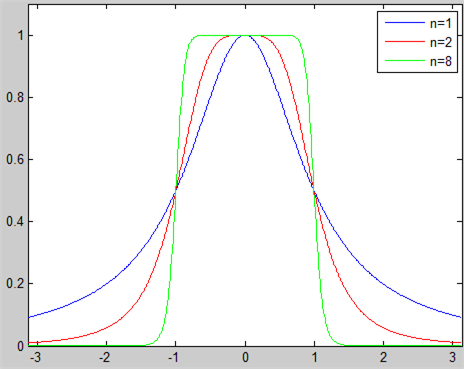
\includegraphics[width=.45\linewidth]{./Figures/butterworth_plot.png}

}

%----------- slide --------------------------------------------------%
\frame
{
\small
%\renewcommand{\theenumi}{\alph{enumi}}
\frametitle{Butterworth Filters-Cont.}

\textcolor{red}{Disadvantages:}\\
\begin{enumerate}
	\item Wide transition region (for low order filters).
	\item Accuracy of approximation cannot be uniformly distributed in PB and SB regions.
\end{enumerate}

\textcolor{red}{Example:} \\
Design a Butterworth LPF, $H_A(s)$, that has attenuation of at least 10dB at $\omega=2\omega_c$ where
$\omega_c = 2.5 \times 10^3$\\ \vspace{.2in}

$A_N(\tilde\omega^2) = \frac{1}{1+\tilde\omega^{2n}}$\\ \vspace{.1in}
$A_N(2^2) = \frac{1}{1+2^{2n}}$\\ \vspace{.1in}
$-10 \log_{10}{|A_N(2^2)|} \ge10\implies (1+2^{2n})\ge 10 \implies n= 1.58 \implies n=2$\\ \vspace{.1in}
From table:  $H_N(s) = \frac{1}{s^2+1.414s+1}$\\ \vspace{.1in}
Denormalize, $s\to s/\omega_c$\\ \vspace{.1in}
$H_A(s) = H_N(\frac{s}{\omega_c}) = \frac{1}{1.6\times 10^{-7}s^2+5.657\times 10^{-4}s+1}$




}

%----------- slide --------------------------------------------------%
\frame
{
\small
%\renewcommand{\theenumi}{\alph{enumi}}
\frametitle{Butterworth Filters-Cont.}

\textcolor{blue}{Short-Cut Method:} \\ \vspace{.1in}
The required filter order for providing a magnitude of $1/A$ (not in dB) at frequency $\omega$ can be obtained using, \vspace{.2in}


\boxed{$$n= \frac{\log_{10} (A^2-1)}{2\log_{10} (\frac{\omega}{\omega_c})}$$} \\ \vspace{.1in}
For previous example, \\ \vspace{.1in}
$-20 \log_{10} 1/A =10 ~dB  \implies A=3.3$ \\ \vspace{.1in}
$n= \frac{\log_{10} (3.3^2-1)}{2\log_{10} 2}=1.653 \implies n=2$ \\ \vspace{.1in}





}

%----------- slide --------------------------------------------------%
\frame
{
%\vspace{-.2in}
\small
%\renewcommand{\theenumi}{\alph{enumi}}
\frametitle{Review of Analog Filters-Cont.}

\textcolor{red}{2. Lowpass Chebyshev Filters}\\
\begin{itemize}
	\item Sharper cutoff or narrower transition region.
	\item Magnitude of error is equiripple over the passband (Type $I$) or over the stopband (Type $II$).
\end{itemize}

\textcolor{red}{Type $I$ Chebyshev:} Magnitude-squared function is given by\\
$A_N(\tilde\omega^2) = |H_N(j\tilde\omega)|^2 = \frac{1}{1+F(\tilde\omega^2)}$\\
where $F(\tilde\omega^2) = \epsilon^2C_n^2(\tilde\omega)$\\
$\epsilon$: Ripple factor (determines ripple in passband)\\
$C_n(\tilde\omega)$:$~n^{th}$ order Chebyshev polynomial\\
$C_n(\tilde\omega) = \cos{(n\cos^{-1}\tilde\omega)}$ for $0\le\tilde\omega\le1$ (passband)\\
$C_n(\tilde\omega) = \cosh{(n\cosh^{-1}\tilde\omega)}$ for $\tilde\omega >1$ (stopband)\\
For any $n$,  $0\le |C_n(\tilde\omega)|\le1$ for $0\le\tilde\omega\le 1$\\
~~~~~~~~~~~~~~~~~~~~$ |C_n(\tilde\omega)|>1$ for $\tilde\omega> 1$\\
$ n=1 \implies C_1(\tilde\omega) = \tilde\omega$\\
$n=2 \implies C_2(\tilde\omega) = 2\tilde\omega^2-1$\\
$n=3 \implies C_3(\tilde\omega) = 4\tilde\omega^3-3\tilde\omega$\\
$\vdots$\\
i.e. $C_n(\tilde\omega)$ is an odd/even polynomial when $n$ is odd/even.

}

%----------- slide --------------------------------------------------%
\frame
{
%\vspace{-.2in}
\small
%\renewcommand{\theenumi}{\alph{enumi}}
\frametitle{Chebyshev Filters-Cont.}

Chebyshev polynomials can be generated recursively using, \\
\boxed{$$C_{n+1}(\tilde\omega)+C_{n-1}(\tilde\omega) = 2\tilde\omega C_n(\tilde\omega)$$}\\
For $n:$ even, ~$C_n^2(0) = 1 \implies A(0) = \frac{1}{1+\epsilon^2}$\\
For $n:$ odd, ~ $C_n^2(0) = 0\implies A(0)  = 1$\\
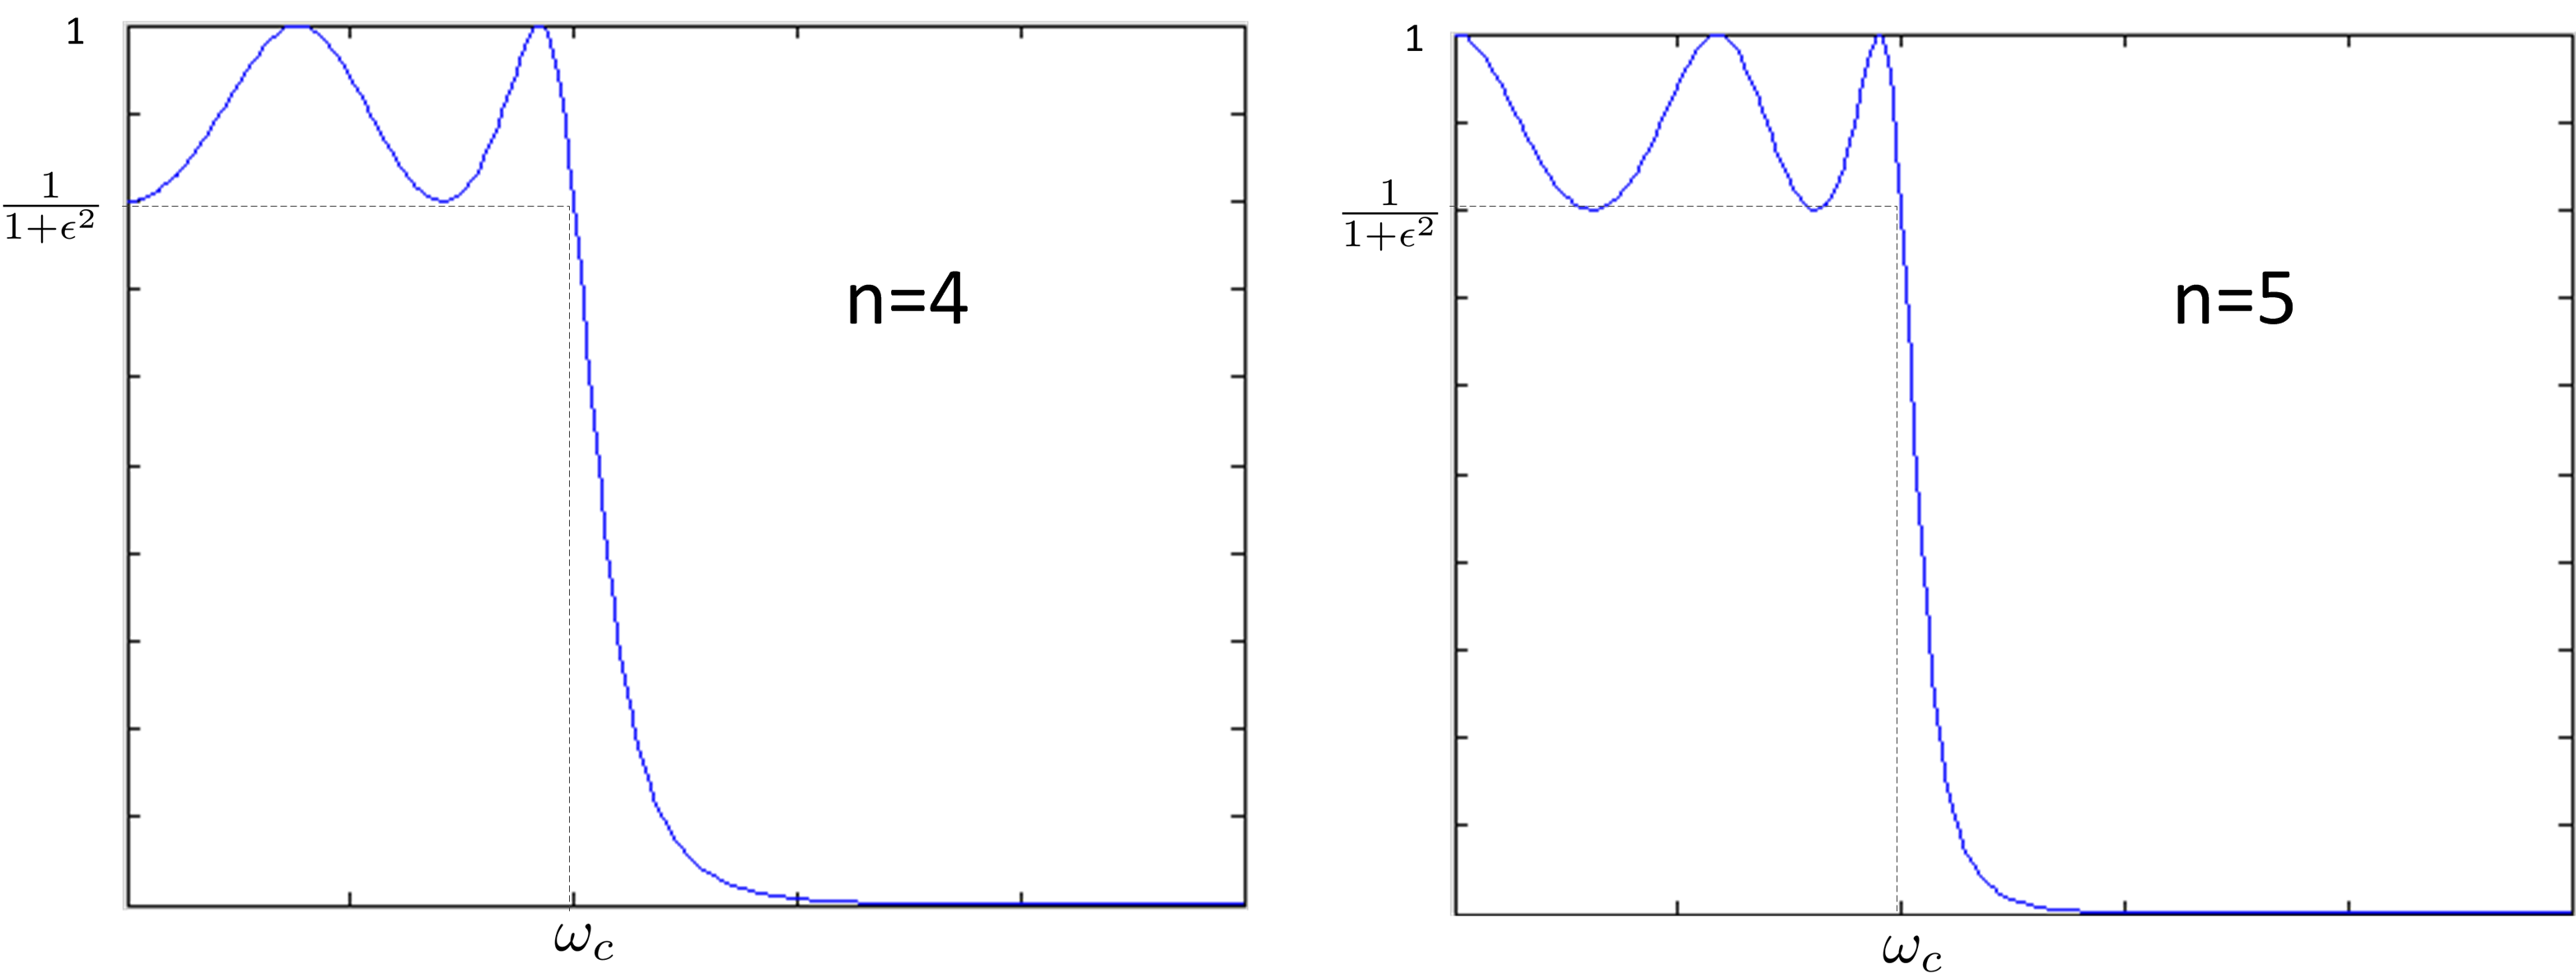
\includegraphics[width=.82\linewidth]{./Figures/cheby_filter.png}\\
$\max |H_N(j\omega)| = A_{max} =1$:  Max gain in passband\\
$\min |H_N(j\omega)| = A_{min} = \frac{1}{\sqrt{1+\epsilon^2}}$: Min gain in passband\\
Define: \\
$r_{dB} = 20 \log_{10} \frac{A_{max}}{A_{min}} = 10 \log_{10}{(1+\epsilon^2)}~~~:$ Loss in passband\\
$r$(peak-to-peak) $= A_{max}-A_{min}=1-\frac{1}{\sqrt{1+\epsilon^2}}$


}

%----------- slide --------------------------------------------------%
\frame
{

\small
%\renewcommand{\theenumi}{\alph{enumi}}
\frametitle{Chebyshev Filters-Cont. }

To find pole locations of the Chebyshev filter, change $\omega=s/j$ and set the denominator to zero, \\ \vspace{.1in}

$1+\epsilon^2C_n^2(s/j)=0 \implies \cos{(n\cos^{-1}(\frac{s}{j}))}=\pm \frac{j}{\epsilon}$ \\ \vspace{.1in}
But, using $s_k=\sigma_k+ j \omega_k$, we get \\ \vspace{.1in}

$\sigma_k =-\sinh \varphi \sin [\frac{(2k-1)\pi}{2n}] ~~ k \in [0,2n-1]$ \\ \vspace{.1in}
$\omega_k =\cosh \varphi \cos [\frac{(2k-1)\pi}{2n}] ~~ k \in [0,2n-1]$ \\ \vspace{.1in}

where \\

$\sinh \varphi= \frac{\gamma-\gamma^{-1}}{2}$ \hspace{.1in} , \hspace{.1in} $\cosh \varphi= \frac{\gamma+\gamma^{-1}}{2}$, and \\
$\gamma = (\frac{1+\sqrt{1+\epsilon^2}}{\epsilon})^{1/n}$. \vspace{.1in}

It is interesting to note that from equations for $\sigma_k$  and $\omega_k$, we have, \\ \vspace{.1in}

$\frac{\sigma^2_k}{\sinh^2 \varphi}+\frac{\omega^2_k}{\cosh^2 \varphi}=1$ \\ \vspace{.14in}

i.e. the poles are located on an ellipse in the $s$-plane.


}

%----------- slide --------------------------------------------------%
\frame
{
%\vspace{-.2in}
\small
%\renewcommand{\theenumi}{\alph{enumi}}
\frametitle{Chebyshev Filters-Cont.}


\textcolor{red}{Example:}\\ \vspace{.05in}
Design a Chebyshev Type $I$ filter with 1dB ripple in passband and attenuation of at least 20dB at $\omega = 2\omega_c$, $f_c = 3 kHz$.\\ \vspace{.05in}

$r = 10 \log_{10} {(1+\epsilon^2)} = 1 \implies \epsilon = .05088$\\ \vspace{.05in}
$-10\log_{10} \frac{1}{1+\epsilon^2C_n^2(2)} \ge 20$\\ \vspace{.05in}
Since in stopband, $\epsilon^2C_n^2(2) \gg1 $\\ \vspace{.06in}
Thus, \\
$10 \log_{10}{\epsilon^2} + 10 \log_{10} {C_n^2(2)} \ge 20$\\ \vspace{.05in}
$\log_{10}{[\cosh(n\cosh^{-1} 2)]} \ge 1- \log_{10} \epsilon = 1.2935 \implies n \cosh^{-1} 2 \ge 3.67 $\\ \vspace{.05in}
or  $ n \ge 2.8 \implies n=3$\\ \vspace{.06in}
Use Table 11.4 (for $r=1dB$)\\ \vspace{.06in}
$H_N(s) = \frac{0.4913}{s^3+0.9883s^2 +1.2384s + 0.4913}$\\ \vspace{.06in}
Denormalize: $\omega_c = 2\pi \times 3 \times 10^3 = 6\pi \times10^3 Rad/Sec$\\ \vspace{.06in}
$s \to \frac{s}{\omega_c}$\\ \vspace{.05in}
$H_A(s) = \frac{0.4913}{1.493 \times 10^{-13}s^3+2.78 \times 10^{-9}s^2+6.569 \times 10^{-5} s + 0.4913}$


}

%----------- slide --------------------------------------------------%
\frame
{
\small
%\renewcommand{\theenumi}{\alph{enumi}}
\frametitle{Review of Analog Filters-Cont.}

\textcolor{blue}{Short-Cut Method:} \\
If the magnitude of minimum stopband loss is $1/A$ at frequency $\omega_r$, then the order can be found using \vspace{.1in}
\boxed{$$n= \frac{\log_{10} (g+\sqrt{g^2-1})}{\log_{10} (\omega_r +\sqrt{\omega_r^2-1})}$$} \\ \vspace{.07in}
where $g=\sqrt{\frac{A^2-1}{\epsilon^2}}$ \vspace{.07in}

\textcolor{red}{3. Elliptic Filters:}\\
Characteristics are:
\begin{enumerate}
	\item Equiripple both in passband and stopband.
	\item Excellent transition region.
\end{enumerate}

The magnitude-squared function for elliptic filters is:\\ \vspace{.1in}
$A(\tilde{\omega}^2) = \frac{1}{1+\epsilon^2R_n^2(\tilde{\omega},\kappa_1)}$\\ \vspace{.1in}
$R_n(\tilde{\omega},\kappa_1): $  Chebyshev rational function with roots that are related to Jacobi elliptic functions hence called \textit{elliptic filters}.\\
$\kappa_1 \triangleq \epsilon/\sqrt{A^2-1}$: selectivity factor\\
}


%----------- slide --------------------------------------------------%
\frame
{
%\vspace{-.2in}
\small
%\renewcommand{\theenumi}{\alph{enumi}}
\frametitle{Elliptic Filters}
Define transition ratio $p = \frac{\omega_c}{\omega_r}$.  Then the order of the elliptic filter to meet $\epsilon, A$ (as defined before) and $\omega_c,\omega_r$ specs is:\\ \vspace{.07in}
$n = \frac{K(p)K(\sqrt{1-\kappa_1^2})}{K(\kappa_1)K(\sqrt{1-p^2})}$\\ \vspace{.06in}
$K(.)$:  Complete elliptic integral of the 1st kind, \\ \vspace{.06in}
$K(x) = \int\limits_0^1 \frac{1}{(1-t^2)^{1/2}(1-xt^2)^{1/2}} dt$ \vspace{.05in}

\textcolor{red}{Remarks:}\\
\begin{enumerate}
	\item In this filter, $\epsilon$ (ripple factor) determines the passband ripple, while the combination of $\epsilon$ and $\kappa_1$ specify the stopband ripple.
	\item To obtain equiripple in both passband and stopband elliptic filters must have poles on $j\omega$ axis.
    \item When  $\kappa_1 \rightarrow \infty$  the elliptic rational function becomes a Chebyshev polynomial, and therefore the filter becomes a Chebyshev Type I filter, with ripple factor $\epsilon$.
\end{enumerate}

\textcolor{red}{Disadvantages:}\\
\begin{enumerate}
	\item Nonlinear phase characteristics.
	\item Delay varies with frequency.
\end{enumerate}

}

%----------- slide --------------------------------------------------%
\frame
{
%\vspace{-.2in}
\normalsize
%\renewcommand{\theenumi}{\alph{enumi}}
\frametitle{Review of Analog Filters-Cont.}
\textcolor{red}{4. Bessel Filters:}\\ \vspace{.05in}
\begin{itemize}
	\item Excellent phase characteristic (nearly linear).
	\item Wide transition region (disadvantage).
	\item Cutoff Frequency changes as function of $n$ (disadvantage).
\end{itemize}
 All-pole filter with transfer function, \\
$H_A(s) = \frac{d_0}{B_n(s)}$\\ \vspace{.05in}
where $B_n(s)$: $n^{th}$ order Bessel Polynomial \\ \vspace{.05in}
  $B_n(s) = \sum\limits_{i=0}^n d_i s^i$\\ \vspace{.05in}
$d_i = \frac{(2n-i)!}{2^{n-i}i!(n-i)!},~~i \in[0,n]$\\ \vspace{.05in}

Bessel polynomials satisfy,  \boxed{$$B_n(s) = (2n-1)B_{n-1}(s) + s^2B_{n-2}(s)$$}\\ \vspace{.05in}
with $B_0(s) = 1,~~~~B_1(s) = s+1$\\ \vspace{.05in}

Cutoff Frequency varies as function of order $n$,
$\omega_c \approx d_0^{1/n}$


}

\section{Digital Filter Design}
%----------- slide --------------------------------------------------%
\frame
{
\vspace{-.8in}
\small
%\renewcommand{\theenumi}{\alph{enumi}}
\frametitle{Recursive Digital Filter Design Using Bilinear $z$-Mapping}

\textbf{Idea:} Analog systems are implemented using integrators, multipliers, and adders. Map every integrator $H_I(s)  = 1/s$ (or $h_I(t) = u_s(t)$)
to the digital domain. \\ \vspace{.08in}

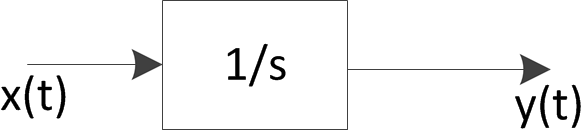
\includegraphics[width=.3\linewidth]{./Figures/bilinear_diag.png} \\
Convolution integral: $y(t) = \int\limits_0^t x(\tau)h_I(t-\tau) d \tau$\\ \vspace{.05in}
Let $0<t_1<t_2$, then \\ \vspace{.05in}
$y(t_2) = \int\limits_0^{t_2} x(\tau)h_I(t-\tau) d \tau$\\ \vspace{.05in}
$y(t_1) = \int\limits_0^{t_1} x(\tau)h_I(t-\tau)d \tau$\\ \vspace{.05in}
$y(t_2)-y(t_1) = \int\limits_{t_1}^{t_2} x(\tau)d \tau = $Area\\ \vspace{.05in}
$\approx \frac{(t_2-t_1)}{2}[x(t_1)+x(t_2)]$ \hspace{.1in} Trapezoidal rule of integration.\\ \vspace{.05in}
Let $t_1 = (n-1)T,~~t_2 = nT$\\ \vspace{.05in}
$y(nT)-y((n-1)T) = \frac{T}{2}[x((n-1)T)+x(nT)]$\\ \vspace{.05in}

\vspace{-2.6in}
\hspace{2.5in}
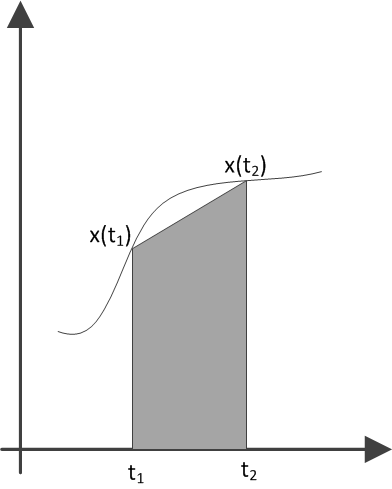
\includegraphics[width=.25\linewidth]{./Figures/trapezoid.png}


}



%----------- slide --------------------------------------------------%
\frame
{
%\vspace{-.8in}
\small
%\renewcommand{\theenumi}{\alph{enumi}}
\frametitle{Bilinear $z$-Mapping-Cont.}

Take $z$-transform:\\ \vspace{.05in}

$Y(z)-z^{-1}Y(z) = \frac{T}{2}[z^{-1}X(z)+X(z)]$\\ \vspace{.05in}
$H_I(z) = \frac{Y(z)}{X(z)} = \frac{T}{2}\frac{(1+z^{-1})}{1-z^{-1}} = \frac{T}{2}\frac{z+1}{z-1}$ \\ \vspace{.05in}

Thus the mapping from $s$-domain to $z$-domain is:\\ \vspace{.05in}
$1/s \to \frac{T}{2}\frac{(z+1)}{(z-1)}$\\ \vspace{.1in}
\boxed{$$s \to \frac{2}{T}\frac{(1-z^{-1})}{(1+z^{-1})}$$}:  \textbf{Bilinear $z$-mapping} \\ \vspace{.1in}
Once $H_A(s)$ prototype is described: \\ \vspace{.1in}
$H_D(z) = H_A(s)|_{s=\frac{2}{T}\frac{(1-z^{-1})}{(1+z^{-1})}}$\\ \vspace{.1in}

\textcolor{red}{Properties of Bilinear $z$-Mapping:}\\ \vspace{.1in}

Recall: $s = \frac{2}{T}\frac{(z-1)}{z+1)}$ or $z = \frac{2/T+s}{2/T-s}$\\ \vspace{.05in}

Also $z=re^{j\Omega}, \text{and} ~s = \sigma+j\omega$ which gives \\
}

%----------- slide --------------------------------------------------%
\frame
{
%\vspace{-.8in}
\normalsize
%\renewcommand{\theenumi}{\alph{enumi}}
\frametitle{Bilinear $z$-Mapping-Properties}


$re^{j\Omega} = \frac{(2/T+\sigma)+j\omega}{(2/T-\sigma)-j\omega}$\\ \vspace{.05in}

Then equations for $r$ and $\Omega$ become, \\ \vspace{.05in}

\boxed{$$r = \left[\frac{(2/T+\sigma)^2+\omega^2}{(2/T-\sigma)^2+\omega^2}\right]^{1/2}$$}\\ \vspace{.05in}
\boxed{$$\Omega = \tan^{-1}{\frac{\omega}{\frac{2}{T}+\sigma}} + \tan^{-1} \frac{\omega}{\frac{2}{T}-\sigma}$$}\\ \vspace{.1in}

Right half of $s$-plane:  $\sigma>0 \implies r>1$:  outside unit circle\\ \vspace{.05in}
On $j\omega$ axis:  $\sigma = 0 \implies r=1$: on unit circle\\ \vspace{.05in}
Left half of $s$-plane:  $\sigma<0 \implies r<1$: inside the unit circle\\ \vspace{.1in}

$\implies$ Stable $H_A(s)$ is mapped to stable $H_D(z)$.\\ \vspace{.05in}

Additionally, it is obvious that $H_D(z)$ will have real coefficients. However, there is an issue
with this mapping called \textit{warping}. \\


}

%----------- slide --------------------------------------------------%
\frame
{
%\vspace{-.8in}
\normalsize
%\renewcommand{\theenumi}{\alph{enumi}}
\frametitle{Bilinear $z$-Mapping-Warping Effects}

For simplicity, let $\sigma = 0$ in equation of $\Omega$, \\ \vspace{.05in}
$\Omega = 2 \tan^{-1} \frac{\omega}{2/T} = 2 \tan^{-1} \frac{\omega T}{2}$\\ \vspace{.05in}
or $\omega = \frac{2}{T} \tan \frac{\Omega}{2}$:  Nonlinear relation between $\Omega, ~\omega$\\ \vspace{.1in}
%Start with $\omega = \frac{2}{T} \tan \frac{\Omega}{2}$\\ \vspace{.05in}
Let $\tilde \Omega = \frac{\Omega}{T}$  (Normalized $\Omega$)\\ \vspace{.08in}
$\omega = \frac{2}{T} \tan \frac{\tilde \Omega T}{2}$\\ \vspace{.08in}
When $\frac{\tilde \Omega T}{2}<0.15,~~\tan \frac{\tilde \Omega T}{2} \approx \frac{\tilde \Omega T}{2} \implies \omega \approx \tilde \Omega$ \\ \vspace{.1in}
i.e.  approximately linear portion of tangent curve. \\ \vspace{.08in}

Thus, If all essential frequencies ($\omega_c, \omega_r$) are below $\tilde \Omega = \frac{0.3}{T}$, no prewarping is needed since minimal warping effects and $\omega \approx \tilde \Omega$. \vspace{.05in}

If not, prewarp the analog filter before bilinear $z$-mapping. \\ \vspace{.05in}


\textbf{Note: }Since $\omega_s=\frac{2 \pi}{T}$ the condition $\tilde \Omega = \frac{0.3}{T}$ can be rewritten as $\tilde \Omega = \frac{0.3}{2 \pi}\omega_s \approx 0.05 \omega_s$ i.e. way below $\omega_s$. 


}


%----------- slide --------------------------------------------------%
\frame
{
%\vspace{-.8in}
\small
%\renewcommand{\theenumi}{\alph{enumi}}
\frametitle{Bilinear $z$-Mapping-Warping Effects}
\textbf{Note: }Warping affects both magnitude and phase responses.  Although, the amplitude distortion caused by warping can be remedied by prewarping, little can be done to linearize the phase except maybe using equalization methods. \\

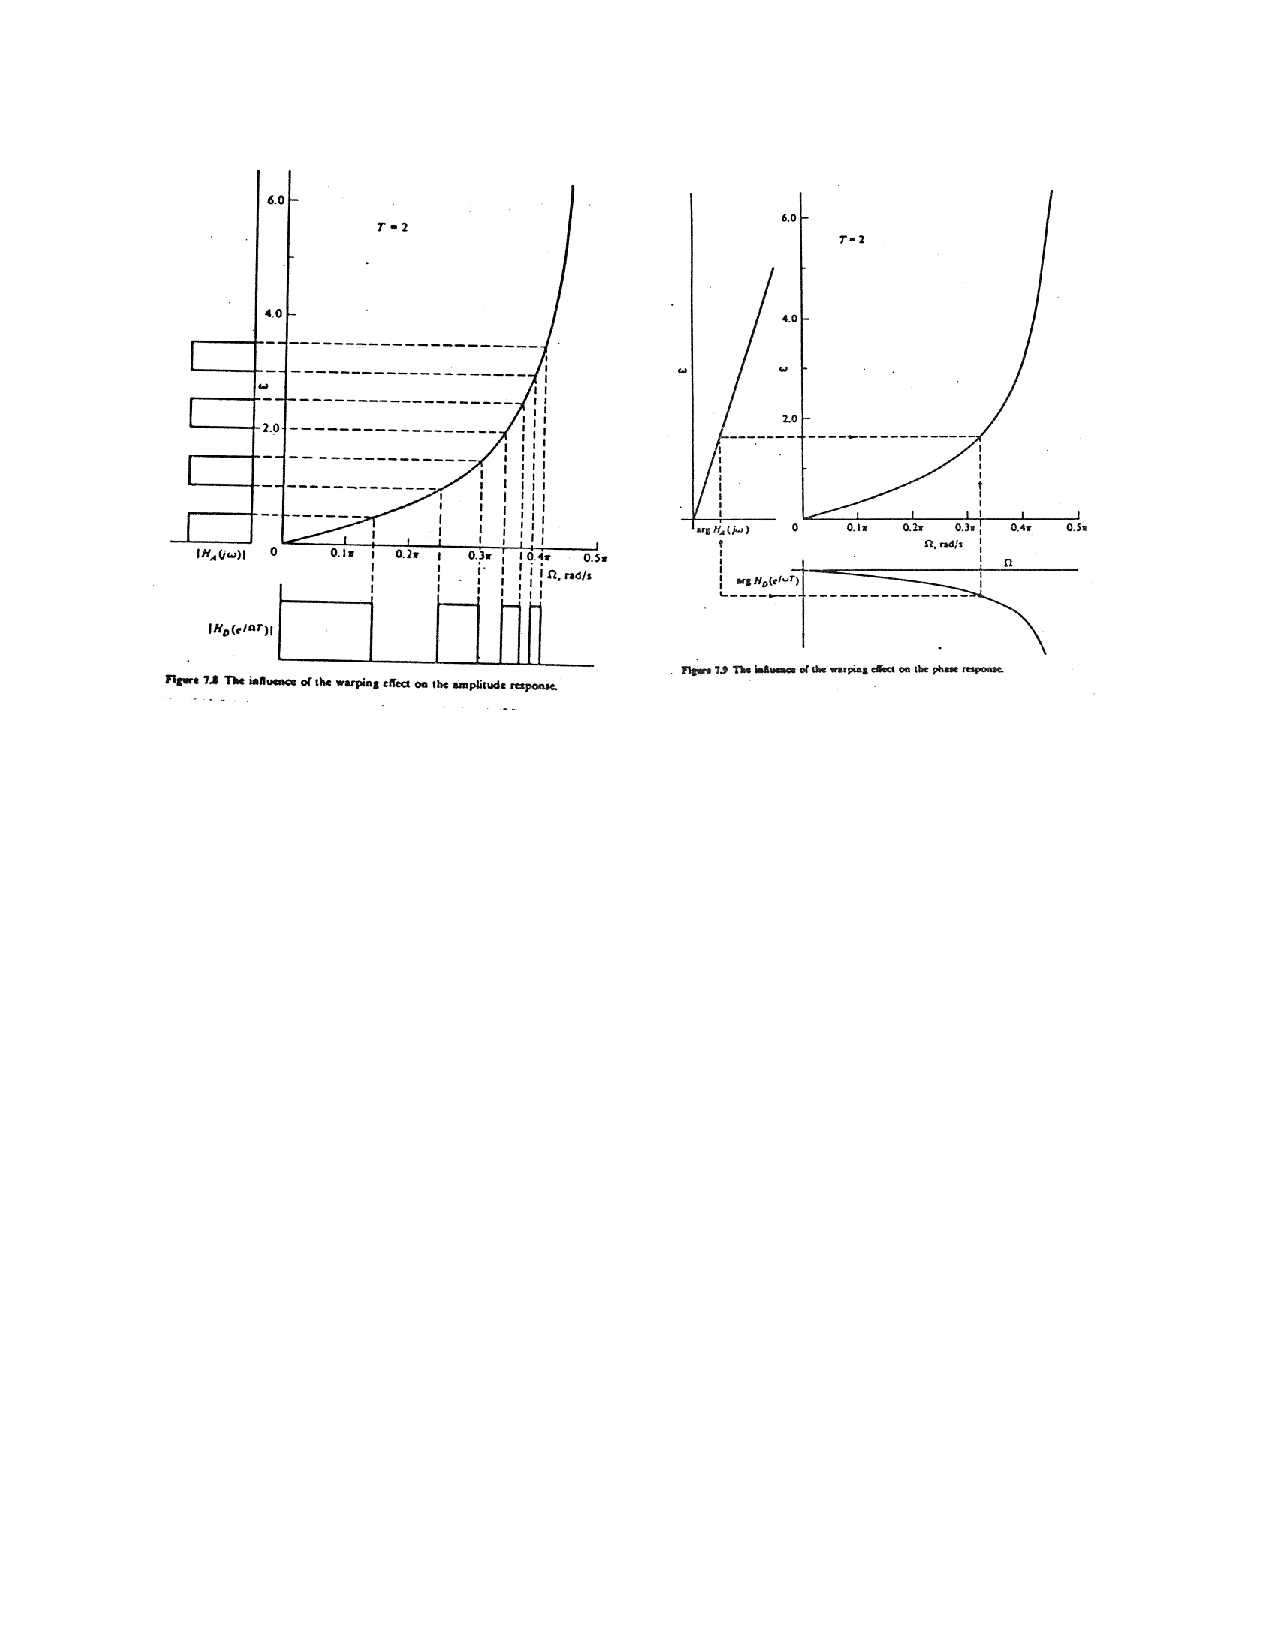
\includegraphics[width=1\linewidth]{./Figures/warping.pdf}


}



%----------- slide --------------------------------------------------%
\frame
{
%\vspace{-.8in}
\small
%\renewcommand{\theenumi}{\alph{enumi}}
\frametitle{Bilinear $z$-Mapping-Prewarping}
\textcolor{red}{Procedure:}\\

If all essential frequencies  are above $\tilde \Omega = \frac{0.3}{T}$, then \\ \vspace{.05in}
\begin{enumerate}
	\item Map all essential digital frequencies $\tilde \Omega_i$ to corresponding analog frequencies using
	$\omega_i = \frac{2}{T} \tan \frac{\tilde \Omega_i T}{2}$
	\item Design $H_A(s)$ using these analog frequencies $\omega_i$'s.
 \item Map $H_A(s)$ to $H_D(z)$ using Bilinear $z$-mapping. \vspace{.1in}
\end{enumerate}

\textcolor{red}{Example:}\\ \vspace{.05in}
Design a digital Butterworth filter that meets:
\begin{enumerate}
	\item $T=50~\mu$ sec.
	\item $\tilde f_c = 4$ kHz or $\tilde \Omega_c = 25.13 \times 10^3$ Rad/sec
	\item At $2 \tilde\Omega_c$ attenuation is $\ge 15dB$
\end{enumerate}

Since $\tilde \Omega_c \gg \frac{0.3}{T} \approx 6000 \implies$ Prewaring is needed\\ \vspace{.05in}

We prewarp both $\tilde{\Omega}_c$ and $2 \tilde\Omega_c$, using
}


%----------- slide --------------------------------------------------%
\frame
{
%\vspace{-.8in}
\small
%\renewcommand{\theenumi}{\alph{enumi}}
\frametitle{Bilinear $z$-Mapping-Cont.}

$\omega_c = \frac{2}{T} \tan \frac{\tilde\Omega_c T}{2} \approx 29.1 \times 10^3$ Rad/sec \\ \vspace{.05in}
$\omega_{15dB} = \frac{2}{T}\tan \frac{2\tilde \Omega_c T}{2} = 123.1 \times 10^3$ Rad/sec \\ \vspace{.1in}

We now use these frequencies to design $H_A(s)$ \\ \vspace{.05in}
$|H_A(j\omega)|^2 = \frac{1}{1+\left(\frac{\omega}{\omega_c}\right)^{2n}}$\\ \vspace{.05in}
$-10 \log_{10} {\left| \frac{1}{1+\left(\frac{123.1}{29.1}\right)^{2n}}\right|} \ge 15dB \implies n\ge 1.2 \implies n=2$\\ \vspace{.05in}
From Table 11.2: \\ \vspace{.05in}
$H_N(s) = \frac{1}{s^2+1.4142s+1}$\\ \vspace{.05in}
Denormalize $s \to s/\omega_c$\\ \vspace{.1in}
$H_A(s) = \frac{(29 \times 10^3)^2}{s^2+41.15 \times 10^3s + (29 \times 10^3)^2}$\\ \vspace{.1in}
$H_D(z) = H_A(s)|_{s = \frac{2}{T}\frac{1-z^{-1}}{1+z^{-1}}} = \frac{2.117+4.234z^{-1}+2.117z^{-2}}{10.232-3.766z^{-1}+2.002z^{-2}}$

}
%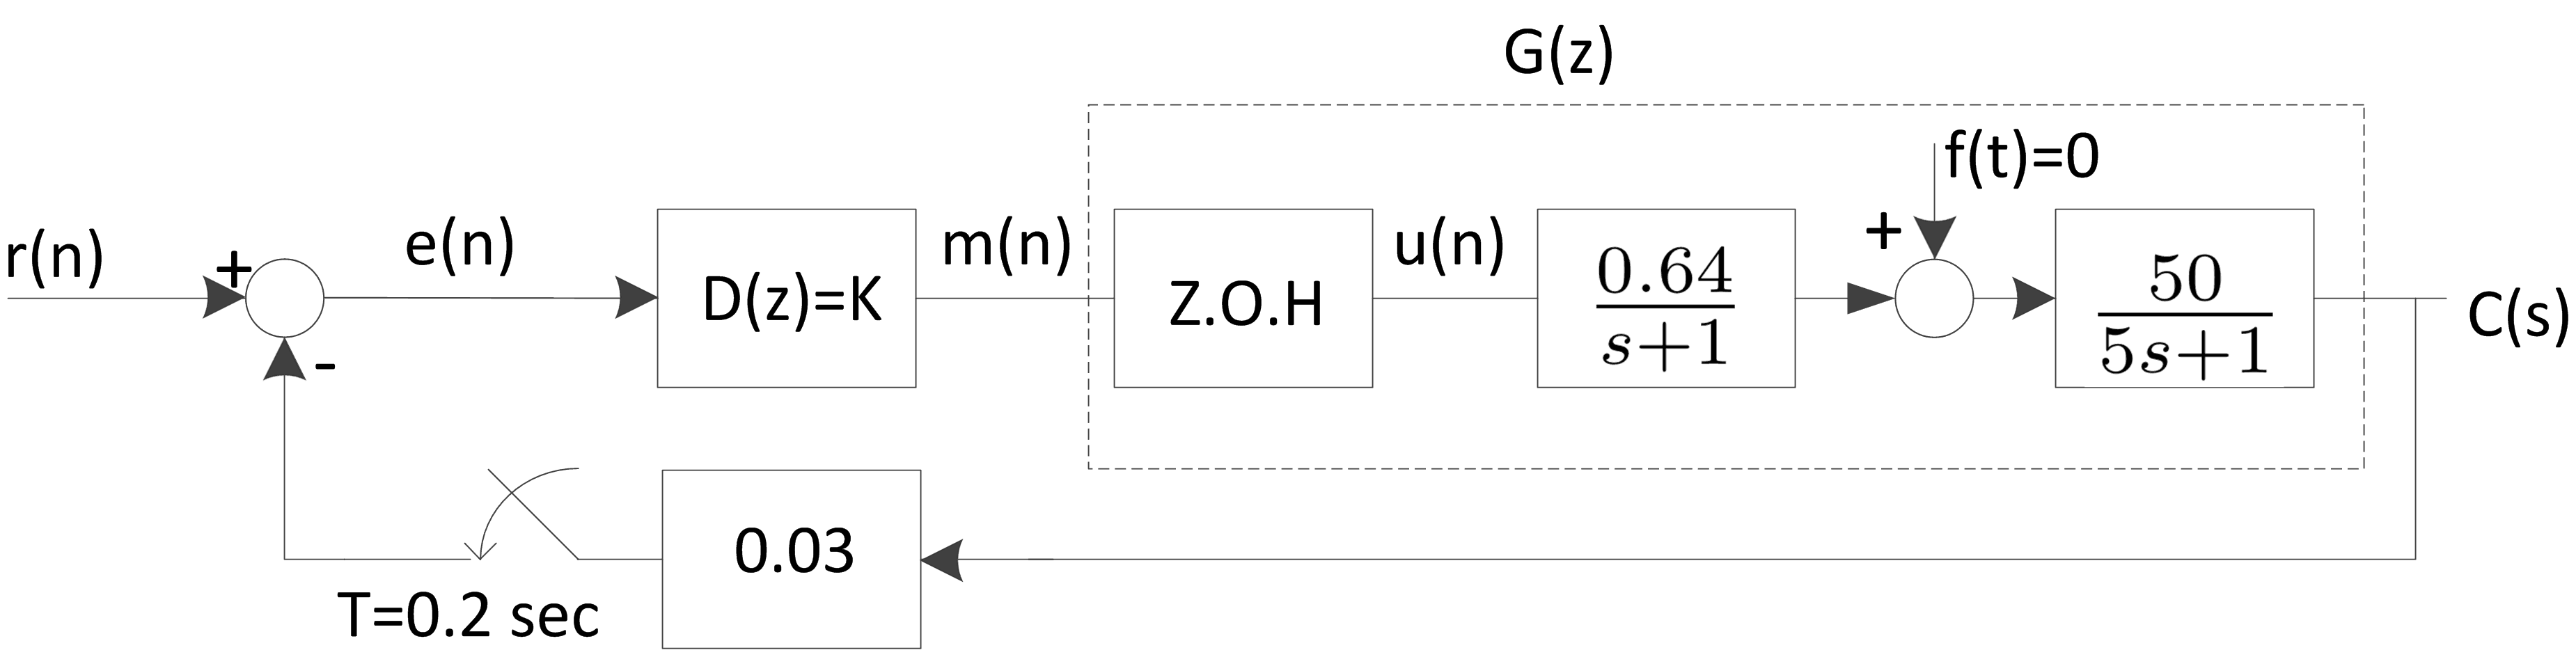
\includegraphics[width=.16\linewidth]{./Figures/example1_diag.png}








\end{document}

